% Created 2016-02-21 Sun 18:53
\documentclass{article}
\usepackage[utf8]{inputenc}
\usepackage[T1]{fontenc}
\usepackage{graphicx}
\usepackage{longtable}
\usepackage{hyperref}
\usepackage{natbib}
\usepackage{amssymb}
\usepackage{amsmath}
\usepackage{geometry}
\geometry{a4paper,left=2.5cm,top=2cm,right=2.5cm,bottom=2cm,marginparsep=7pt, marginparwidth=.6in}
\usepackage[utf8]{inputenc}
\usepackage[T1]{fontenc}
\usepackage{fixltx2e}
\usepackage{graphicx}
\usepackage{grffile}
\usepackage{longtable}
\usepackage{wrapfig}
\usepackage{rotating}
\usepackage[normalem]{ulem}
\usepackage{amsmath}
\usepackage{textcomp}
\usepackage{amssymb}
\usepackage{capt-of}
\usepackage{hyperref}
\author{Jeffrey Skonhovd}
\date{2016-02-19}
\title{Reinforcement Learning: Midterm Project}
\hypersetup{
 pdfauthor={Jeffrey Skonhovd},
 pdftitle={Reinforcement Learning: Midterm Project},
 pdfkeywords={},
 pdfsubject={},
 pdfcreator={Emacs 24.5.1 (Org mode 8.3.3)}, 
 pdflang={English}}
\begin{document}

\maketitle
\tableofcontents



\section{Introduction}
\label{sec:orgheadline1}
   In the course of this class, one of the primary reinforcement learning
algorithms we have studied is \(TD(\lambda)\). In this report, we will review and
attempt to implement portions of Richard Sutton's 1988 paper called Learning to
Predict by the Methods of Temporal Differences. Our focus will be an
implementation of the \(TD(\lambda)\) algorithm and the reproduction of
figures 3, 4 and 5 from the paper. 

\section{Temporal Differences}
\label{sec:orgheadline2}
In this section, I will attempt to give a quick overview of how
Temporal Difference Learning algorithms work and what advantages they
might have over other algorithms. A major advantage that TD procedures
have is the ability to be implemented incrementally. This gives the
algorithms advantages over other methods like supervised learning
since they require far less computational power.

A confusing part of the paper was the introduction of the variable
\(\omega\). \(\omega\) stands for the a vector of modifiable weights. This
\(\omega\) helps us keep track of the changes through the incremental
sequences. A sequence is a change in state off the mdp that we are
attempting to model.  After each sequence we observe, we will generate an
observation \(\Delta\omega_{t}\). This process can be observed in the
following equation, which was equation one in the paper.

\begin{equation}
\omega \leftarrow \omega + \sum_{t=1}^{m}\Delta\omega_{t}
\end{equation}

\(TD(\lambda)\) is a class of \(TD\) procedures that make greater alterations to
more recent predictions. In particular, we know that \(TD(\lambda)\)
will consider exponential weighting with recency. \(TD(\lambda)\) is
given by equation 4 from the paper which is stated below. 

\begin{equation}
\Delta\omega_{t} = \alpha(P_{t+1} - P_{t})\sum_{k=1}^{T} \lambda^{t-k}\nabla_{\omega}P_{k}
\end{equation}

\section{Experments Replicated}
\label{sec:orgheadline10}

\subsection{Overview of Bounded Random Walk Problem}
\label{sec:orgheadline3}
The experiments were conducted on a simple dynamical system that
generates bounded random walks. Bound random walks take random steps
either left or right until the sequence hits a boundary. The movements
left or right are both equally probable in our example. We describe
the possible states will the letters \(A-G\). The bounds can be
arbitrary, but for this example the left side will be A, and the right 
side is G.

\subsection{Expirement Data}
\label{sec:orgheadline4}
Sutton's paper gives good instructions on how to construct the
training sets, however he is ambiguous on certain details. In order to
replicate the experiment, I randomly generated 100 training sets, each
containing 10 sequences. A sequence is the set of states that the mdp
will go through until the mdp ends at a bound. For example, the
following is a sequnce, DEFEDEDEFG. The much
longer string DEFEDCDEFEFEDEFEDEFEDCDCDCBCDCDCBCDEDCBA would be
considered a sequence as  well. For these experiments, Sutton does not
state a limit to the length of a sequence, or a minimum for the
sequence. 

Now as I explained above, \(TD(\lambda)\) makes greater alterations
to more recent predictions. We know from equation 4, that the exponent
on lambda will get large as we get farther along in the sequence. Now
in the case of \(TD(1)\), we know that 1 rasied to any power is 1. So in
that case every member of the sequence would be weighted the same. So
would a distribution of training sets with longer sequences effect our
results? 

\subsection{Experiment 1}
\label{sec:orgheadline6}
We used the training sets described above for experiments one. But, we
do not update the weight vector after each sequence as indicated by
our equation \((1)\). Instead, we perform what the paper calls the
repeated presentations training paradigm. We keep iterating through
the training set until we no longer see a change in
\(\Delta\omega\). Once we converge, we will get the RSME error between
our weights and the ideal weights. The ideal weights are
\([\frac{1}{6},\frac{1}{3},\frac{1}{2},\frac{2}{3},\frac{5}{6}]\).
\subsubsection{Figure 3}
\label{sec:orgheadline5}
The following is our replication of Figure 3. This graph shows the
average RMSE error over the 100 test cases versus the increasing value
for lambda. We assume that the weights are initially set with random
weights. 

\begin{center}
\begin{tabular}{l}
\hline
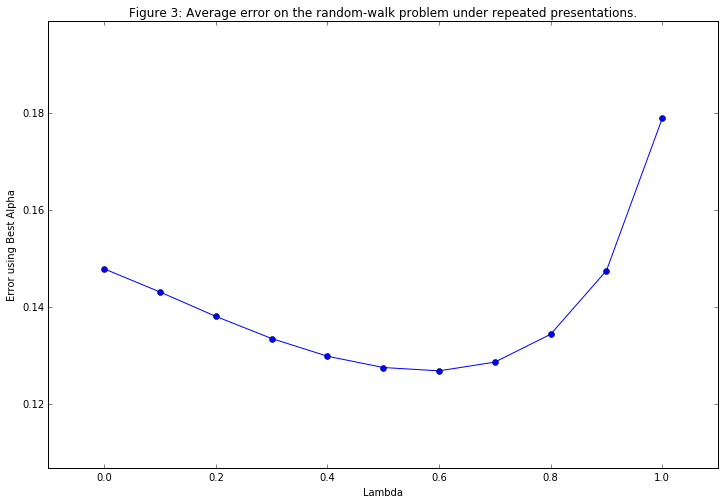
\includegraphics[width=.9\linewidth]{figure3_1.png}\\
\\
\end{tabular}
\end{center}

\subsection{Experiment 2}
\label{sec:orgheadline9}
The second experiment will examine the learning rate when we only view
the training set exactly once. We only show each training set only
onces, and weights are updated like the equation \((1)\). We also use a
range of alpha values, instead of defaulting to \(0.01\) like in
experiment one. We also will default the value of \(\omega\) to \([0.5,
0.5, 0.5, 0.5, 0.5]\).
\subsubsection{Figure 4}
\label{sec:orgheadline7}
The following is our replication for figure 4. This figure shows the
average error on a random walk after experiencing 10 sequences, or one
training set. The \(\lambda = 1\) is the Widrow-Hoff supervised-learning
procedure.
\begin{center}
\begin{tabular}{l}
\hline
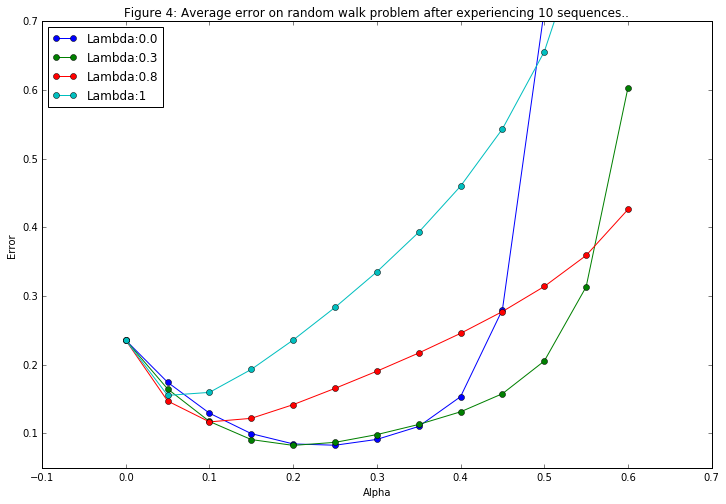
\includegraphics[width=.9\linewidth]{figure4_1.png}\\
\\
\end{tabular}
\end{center}
\subsubsection{Figure 5}
\label{sec:orgheadline8}
THe following is our replication of Figure 5 from the paper. This
figure shows the best error level achieved for each \(\lambda\) 
value. We pulled the best lambda values from the data of figure 4 to
yield the lowest error for that lambda value. 
\begin{center}
\begin{tabular}{l}
\hline
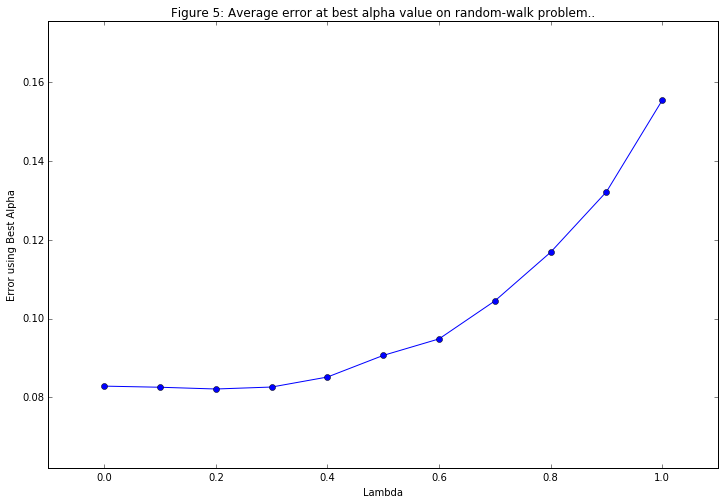
\includegraphics[width=.9\linewidth]{figure5_1.png}\\
\\
\end{tabular}
\end{center}

\section{Conclusion}
\label{sec:orgheadline15}

\subsection{How well do our results match the Paper?}
\label{sec:orgheadline11}
We were significantly happy with our results even if our results where not exact.
We could easily observe the trends in figures 4, 5, and 6. Are their
signficant differences in our Results compared to the Paper? Yes, we
did observe some differences. 

Figure 3 was probably our most accurate graph when concerning change
in error as compared to the paper. However, our std was only around
0.02 for each iteration. we do notice a small in error in from 0.0 to
0.6 then a more signficant rise toward the end.

For figure 4, we notice while alpha is smaller our graph is more
accurate. We do have very large error for \(\lambda = 1\), and \(\lambda
= 0\) for \(\alpha > 0.5\). However, we are happy that the increases in
error as \(\alpha\) is increased are in sync with the paper. \(\lambda
=1\) increases first, followed by \(\lambda = 0.8\), then \(\lambda = 0\)
and finally \(\lambda = 0.3\).

The last figure we will examine is figure 5.  We also had slightly
better error results for each value of lambda, as compared to our
paper. For example, we can see our value at \(\lambda = 0\) has an average error of
0.08 compared to 0.11. If you look at \(\lambda = 1\), we received an
error around 0.16 compared to arround 0.21 for the paper. In general,
I am happy that we achieved a simlar slope of the graph as compared to
the paper.


\subsection{Any pitfalls observed trying to replicate the experiment from the paper?}
\label{sec:orgheadline12}
There was considerable confusion for me to implement experiment 1. I
initially implemented that expirement as what eventually became
experiment 2. I also had trouble picking a correct \(\alpha\) for
experiment 1. I initally thought that 0.10 was a small \(\alpha\), however
I actually got convergence once I picked 0.01. 

\subsection{What steps did you take to overcome those pitfalls?}
\label{sec:orgheadline13}
I generally got through any pitfalls by trial and error. We needed a
small alpha value in experiment one, otherwise we wouldn't
converge. We would get very large differences between the weights. 

\subsection{What assumptions did you make, and why?}
\label{sec:orgheadline14}
We made a couple major assumptions. We do not believe that a minimum
or maximum length of a sequence is set by the paper. However, we do believe it is
reasonable to assume a random distribution of lengths.

For inital values, there was some leeway as Sutton didn't explictly
state some of those values.  We assumed that \(\Delta\omega\) is
initally set to \([0,0,0,0,0]\). Also in experiment one, I assumed that
the \(\omega\) vector could be set to random weights [0 - 1]. 

Are these assumptions justified? I would believe so. We generally
needed to make some guesses to make the algorithm even work. I think
Sutton would have told if the length of a sequence was
specfic. \(\Delta\omega\) should start out at \([0,0,0,0,0]\), otherwise
the algorithm might not converge. 
\end{document}